%!TEX program = xelatex
% ==============================================================================
% AA CONFIGURAZIONE DI BASE ED ENGINE
% ==============================================================================
% BB CLASSE DEL DOCUMENTO
\documentclass[11pt, a4paper]{article}

% ==============================================================================
% AA LINGUA, FONT E TIPOGRAFIA
% ==============================================================================
% BB GESTIONE FONT XELATEX
\usepackage{fontspec}
\setmainfont{Latin Modern Roman}

% BB LOCALIZZAZIONE LINGUISTICA
\usepackage[italian]{babel}

% BB TIPOGRAFIA E MICRO-ESTENSIONI
\usepackage[protrusion=true]{microtype}
\raggedbottom

% ==============================================================================
% AA LAYOUT DI PAGINA E SPAZIATURA PARAGRAFI
% ==============================================================================
% BB GEOMETRIA DEI MARGINI
\usepackage[left=2.4cm, right=1.6cm, top=2cm, bottom=2cm]{geometry}

% BB CONTROLLO SPAZIATURA TRA PARAGRAFI
\usepackage[skip=3pt plus 1pt minus 1pt]{parskip}

% ==============================================================================
% AA MOTORE DEI COLORI E MACRO LOCALI
% ==============================================================================
% BB CARICAMENTO CORE XCOLOR IN SPAZIO GRAY PURO
\usepackage[gray]{xcolor}
% BB MACRO PER I SIGMA MONOCROMATICI
\newcommand{\sigA}{\boldsymbol{\sigma_A}}
\newcommand{\sigB}{\boldsymbol{\sigma_B}}
\newcommand{\sigC}{\boldsymbol{\sigma_C}}

% ==============================================================================
% AA MATEMATICA E SIMBOLI SCIENTIFICI
% ==============================================================================
% BB PACCHETTI MATEMATICI UNICODE
\usepackage{mathtools}
\usepackage[warnings-off={mathtools-overbracket,mathtools-colon}]{unicode-math}
\setmathfont{Latin Modern Math}

% BB METRICHE MATRICI E FORMULE DISPLAY
\setlength{\arraycolsep}{10pt}
\setlength{\abovedisplayskip}{3pt plus 1pt minus 1pt}
\setlength{\belowdisplayskip}{3pt plus 1pt minus 1pt}
\setlength{\abovedisplayshortskip}{0pt plus 1pt}
\setlength{\belowdisplayshortskip}{2pt plus 1pt minus 1pt}
\allowdisplaybreaks

% ==============================================================================
% AA GRAFICA ED ELEMENTI FLOTTANTI
% ==============================================================================
% BB MOTORE DI INCLUSIONE GRAFICA E GESTIONE RIGIDA
\usepackage{graphicx}
\graphicspath{{./E4_2_Images/}}
\usepackage{float}

% ==============================================================================
% AA TITOLI E STRUTTURA DEL DOCUMENTO (MONOCROMATICI NERI)
% ==============================================================================
% BB PACCHETTO TITLESEC
\usepackage{titlesec}

% BB FORMATTAZIONE TIPOGRAFICA (TITOLI NERI)
\titleformat{\section}{\normalfont\Large\bfseries}{\thesection}{1em}{}
\titleformat{name=\section,numberless}{\normalfont\Large\bfseries}{}{0pt}{}
\titleformat{\subsection}{\normalfont\large\bfseries}{\thesubsection}{1em}{}
\titleformat{name=\subsection,numberless}{\normalfont\large\bfseries}{}{0pt}{}
\titleformat{\subsubsection}{\normalfont\normalsize\bfseries}{\thesubsubsection}{1em}{}
\titleformat{name=\subsubsection,numberless}{\normalfont\normalsize\bfseries}{}{0pt}{}

% BB SPAZIATURA VERTICALE DEI TITOLI
\titlespacing*{\section}{0pt}{1.2ex plus 0.4ex minus 0.2ex}{0.6ex plus 0.2ex}
\titlespacing*{\subsection}{0pt}{1ex plus 0.3ex minus 0.2ex}{0.5ex plus 0.2ex}
\titlespacing*{\subsubsection}{0pt}{0.8ex plus 0.2ex minus 0.1ex}{0.4ex plus 0.1ex}

% ==============================================================================
% AA INTEGRAZIONE AMBIENTE MATLAB
% ==============================================================================
% BB CARICAMENTO PACCHETTO MATLAB
\usepackage{matlab}

% BB ATTIVAZIONE SEGNALIBRI E INDICE MATLAB
\matlabmultipletitles
\matlabhastoc

% ==============================================================================
% AA IPERTESTO, SEGNALIBRI ED ELENCHI
% ==============================================================================
% BB CONFIGURAZIONE HYPERREF E METADATI PDF
\hypersetup{
    hidelinks,
    pdfauthor={Francesco Lo Verde},
    pdftitle={Cinematica diretta manipolatore SCARA}
}

% BB SEGNALIBRI AVANZATI
\usepackage{bookmark}

% BB FORMATTAZIONE ELENCHI PUNTATI E NUMERATI
\usepackage{enumitem}
\setlist{itemsep=3.5pt plus 1pt minus 1pt, topsep=4pt plus 1pt minus 1pt, partopsep=0pt, parsep=1pt}

\begin{document}


\matlabtitle{Calcolo cinematica diretta manipolatore SCARA}

\begin{par}
\begin{flushleft}
L'obiettivo della cinematica diretta è determinare la posizione e l'orientamento dell'organo terminale (end-effector) a partire dai valori delle variabili di giunto. Si utilizza la convenzione di Denavit-Hartenberg (DH) per modellare la geometria del robot. La convenzione di Denavit-Hartenberg è un metodo standard per assegnare sistemi di riferimento ai bracci di un robot. Per ogni braccio, si definiscono quattro parametri che descrivono la trasformazione geometrica rispetto al braccio precedente.
\end{flushleft}
\end{par}

\begin{par}
\begin{flushleft}
Si inizia definendo le variabili simboliche necessarie per i parametri DH. Questo permette di eseguire i calcoli in forma generale, senza dover specificare subito valori numerici. Successivamente, si assemblano questi parametri in una tabella dove ogni riga corrisponde a un giunto del robot e le colonne rappresentano i parametri $\left(\begin{array}{c}
\theta ,d,\alpha ,a
\end{array}\right)$.
\end{flushleft}
\end{par}

\begin{matlabcode}
clc;
clear;
close all;

% Definizione variabili simboliche
syms q1 q2 q3 q4 d1 d4 a1 a2 real;

% Tabella parametri Denavit-Hartenberg (DH)
% Le colonne sono: [theta, d, alpha, a]
DH_table = [q1, d1, 0,  a1;
            q2, 0,  pi, a2;
            0,  q3, 0,  0;
            q4, d4, 0,  0];

% Numero giunti manipolatore
n = size(DH_table, 1);
\end{matlabcode}

\begin{par}
\begin{flushleft}
A partire dalla tabella DH, si può calcolare la matrice di trasformazione omogenea $^{i-1}A_i$ per ciascun link $i$. Questa matrice, di dimensioni $4\times 4$, rappresenta la trasformazione (rotazione e traslazione) dal sistema di riferimento del link $i$ a quello del link $i-1$. Si utilizza la funzione \texttt{Compute\_DH\_Transformations} per generare le matrici simboliche per ogni riga della tabella DH.
\end{flushleft}
\end{par}

\begin{matlabcode}
[A_matrices, R_matrices] = Compute_DH_Transformations(DH_table);

for i = 1:n
    fprintf('Matrice di trasformazione omogenea ^(%d)A_(%d):\n', i-1, i);
    disp(A_matrices(:,:,i));
end
\end{matlabcode}
\begin{matlaboutput}
Matrice di trasformazione omogenea ^(0)A_(1):
\end{matlaboutput}
\begin{matlabsymbolicoutput}
\hskip1em $\displaystyle \left(\begin{array}{cccc}
\cos \left(q_1 \right) & -\sin \left(q_1 \right) & 0 & a_1 \,\cos \left(q_1 \right)\\
\sin \left(q_1 \right) & \cos \left(q_1 \right) & 0 & a_1 \,\sin \left(q_1 \right)\\
0 & 0 & 1 & d_1 \\
0 & 0 & 0 & 1
\end{array}\right)$
\end{matlabsymbolicoutput}
\begin{matlaboutput}
Matrice di trasformazione omogenea ^(1)A_(2):
\end{matlaboutput}
\begin{matlabsymbolicoutput}
\hskip1em $\displaystyle \left(\begin{array}{cccc}
\cos \left(q_2 \right) & \sin \left(q_2 \right) & 0 & a_2 \,\cos \left(q_2 \right)\\
\sin \left(q_2 \right) & -\cos \left(q_2 \right) & 0 & a_2 \,\sin \left(q_2 \right)\\
0 & 0 & -1 & 0\\
0 & 0 & 0 & 1
\end{array}\right)$
\end{matlabsymbolicoutput}
\begin{matlaboutput}
Matrice di trasformazione omogenea ^(2)A_(3):
\end{matlaboutput}
\begin{matlabsymbolicoutput}
\hskip1em $\displaystyle \left(\begin{array}{cccc}
1 & 0 & 0 & 0\\
0 & 1 & 0 & 0\\
0 & 0 & 1 & q_3 \\
0 & 0 & 0 & 1
\end{array}\right)$
\end{matlabsymbolicoutput}
\begin{matlaboutput}
Matrice di trasformazione omogenea ^(3)A_(4):
\end{matlaboutput}
\begin{matlabsymbolicoutput}
\hskip1em $\displaystyle \left(\begin{array}{cccc}
\cos \left(q_4 \right) & -\sin \left(q_4 \right) & 0 & 0\\
\sin \left(q_4 \right) & \cos \left(q_4 \right) & 0 & 0\\
0 & 0 & 1 & d_4 \\
0 & 0 & 0 & 1
\end{array}\right)$
\end{matlabsymbolicoutput}
\begin{matlabcode}

T04 = A_matrices(:,:,1) * A_matrices(:,:,2) * A_matrices(:,:,3) * A_matrices(:,:,4);
T04 = simplify(T04);

fprintf('Matrice di trasformazione omogenea totale ^(0)T_(4):\n');
disp(T04);
\end{matlabcode}
\begin{matlaboutput}
Matrice di trasformazione omogenea totale ^(0)T_(4):
\end{matlaboutput}
\begin{matlabsymbolicoutput}
\hskip1em $\displaystyle \left(\begin{array}{cccc}
\cos \left(q_1 +q_2 -q_4 \right) & \sin \left(q_1 +q_2 -q_4 \right) & 0 & a_2 \,\cos \left(q_1 +q_2 \right)+a_1 \,\cos \left(q_1 \right)\\
\sin \left(q_1 +q_2 -q_4 \right) & -\cos \left(q_1 +q_2 -q_4 \right) & 0 & a_2 \,\sin \left(q_1 +q_2 \right)+a_1 \,\sin \left(q_1 \right)\\
0 & 0 & -1 & d_1 -d_4 -q_3 \\
0 & 0 & 0 & 1
\end{array}\right)$
\end{matlabsymbolicoutput}
\begin{par}
\begin{flushleft}
La matrice di trasformazione omogenea totale $^0 T_4$ contiene tutte le informazioni sulla posa dell'organo terminale. Da essa si possono estrarre due elementi chiave:
\end{flushleft}
\end{par}

\begin{itemize}
   \item La \textbf{matrice di rotazione R}, che definisce l'orientamento dell'organo terminale rispetto alla base. Corrisponde alla sottomatrice 3x3 in alto a sinistra.
   \item Il \textbf{vettore di posizione p}, che indica la posizione dell'origine del sistema di riferimento dell'organo terminale. Corrisponde alle prime tre righe della quarta colonna.
\end{itemize}

\begin{matlabcode}
% Estrazione vettore posizione
p04 = T04(1:3, 4);
p04 = simplify(p04);
fprintf('Vettore posizione ^(0)p_(4):\n');
disp(p04);
\end{matlabcode}
\begin{matlaboutput}
Vettore posizione ^(0)p_(4):
\end{matlaboutput}
\begin{matlabsymbolicoutput}
\hskip1em $\displaystyle \left(\begin{array}{c}
a_2 \,\cos \left(q_1 +q_2 \right)+a_1 \,\cos \left(q_1 \right)\\
a_2 \,\sin \left(q_1 +q_2 \right)+a_1 \,\sin \left(q_1 \right)\\
d_1 -d_4 -q_3
\end{array}\right)$
\end{matlabsymbolicoutput}

\begin{matlabcode}
% Estrazione matrice rotazione
R04 = T04(1:3, 1:3);
R04 = simplify(R04);
fprintf('Matrice di rotazione ^(0)R_(4):\n');
disp(R04);
\end{matlabcode}
\begin{matlaboutput}
Matrice di rotazione ^(0)R_(4):
\end{matlaboutput}

\begin{matlabsymbolicoutput}
\hskip1em $\displaystyle \left(\begin{array}{ccc}
\cos \left(q_1 +q_2 -q_4 \right) & \sin \left(q_1 +q_2 -q_4 \right) & 0\\
\sin \left(q_1 +q_2 -q_4 \right) & -\cos \left(q_1 +q_2 -q_4 \right) & 0\\
0 & 0 & -1
\end{array}\right)$
\end{matlabsymbolicoutput}
\newpage
\begin{par}
\begin{flushleft}
Per visualizzare una configurazione specifica del robot sono necessari dei valori numerici. Si sostituiscono ora le variabili simboliche (angoli di giunto e parametri geometrici) con valori numerici.
\end{flushleft}
\end{par}

\begin{matlabcode}
% Lista variabili simboliche
symsList = [q1, q2, q3, q4, d1, d4, a1, a2];
disp('Variabili simboliche:');
disp(symsList);
\end{matlabcode}
\begin{matlaboutput}
Variabili simboliche:
\end{matlaboutput}

\begin{matlabsymbolicoutput}
\hskip1em $\displaystyle \left(\begin{array}{cccccccc}
q_1  & q_2  & q_3  & q_4  & d_1  & d_4  & a_1  & a_2
\end{array}\right)$
\end{matlabsymbolicoutput}
\begin{matlabcode}

% Valori numerici da sostituire
value = [pi/4, pi/3, 0.5, pi/6, 1, 0.2, 0.8, 0.6];

% Sostituzione matrice per matrice
A_Num = zeros(4,4,n);
for i = 1:n
    A_Num(:,:,i) = double(subs(A_matrices(:,:,i), symsList, value));
end

T04_Num = double(subs(T04, symsList, value));
fprintf('Matrice di trasformazione omogenea ^(0)T_(4) numerica:\n');
disp(T04_Num);

% Stampa matrici numeriche
for i = 1:n
    fprintf('Matrice ^(%d)A_(%d) numerica:\n', i-1, i);
    disp(A_Num(:,:,i));
end
\end{matlabcode}
\begin{matlaboutput}
Matrice di trasformazione omogenea ^(0)T_(4) numerica:
    0.2588    0.9659         0    0.4104
    0.9659   -0.2588         0    1.1452
         0         0   -1.0000    0.3000
         0         0         0    1.0000
Matrice ^(0)A_(1) numerica:
    0.7071   -0.7071         0    0.5657
    0.7071    0.7071         0    0.5657
         0         0    1.0000    1.0000
         0         0         0    1.0000
Matrice ^(1)A_(2) numerica:
    0.5000    0.8660         0    0.3000
    0.8660   -0.5000         0    0.5196
         0         0   -1.0000         0
         0         0         0    1.0000
Matrice ^(2)A_(3) numerica:
    1.0000         0         0         0
         0    1.0000         0         0
         0         0    1.0000    0.5000
         0         0         0    1.0000
Matrice ^(3)A_(4) numerica:
    0.8660   -0.5000         0         0
    0.5000    0.8660         0         0
         0         0    1.0000    0.2000
         0         0         0    1.0000
\end{matlaboutput}

\newpage
\matlabheadingtwo{Visualizzazione grafica manipolatore SCARA}

\begin{matlabcode}
fig_name    = 'Configurazione manipolatore SCARA';
arrow_scale = 0.12;
view_angles = [105, 22];
labels      = {'Terna 0 (base)', 'Terna 1', 'Terna 2', 'Terna 3', 'Terna 4 (EE)'};

figure('Name', fig_name, 'Color', 'w');
hold on;
grid on;
box on;
xlabel('X [m]', 'FontWeight', 'bold');
ylabel('Y [m]', 'FontWeight', 'bold');
zlabel('Z [m]', 'FontWeight', 'bold');
view(view_angles(1), view_angles(2));
axis equal;

% 1. Calcolo di tutte le posizioni e orientamenti (base + n giunti)
T_cumulative = eye(4);
positions = zeros(n+1, 3);
R_all     = zeros(3, 3, n+1);
positions(1, :) = T_cumulative(1:3, 4).';
R_all(:, :, 1)  = T_cumulative(1:3, 1:3);

for i = 1:n
    T_cumulative = T_cumulative * double(A_Num(:, :, i));
    positions(i+1, :) = T_cumulative(1:3, 4).';
    R_all(:, :, i+1)  = T_cumulative(1:3, 1:3);
end

% 2. Disegno bracci
h_link = plot3(positions(:,1), positions(:,2), positions(:,3), '-', 'Color', [0.25 0.25 0.25], ...
    'LineWidth', 2.5);

% 3. Evidenziazione giunti meccanici ed end-effector
h_base = plot3(positions(1,1), positions(1,2), positions(1,3), 's', 'MarkerSize', 8, ...
    'MarkerFaceColor', [0.4 0.4 0.4], 'MarkerEdgeColor', 'k');
h_joints = plot3(positions(2:end-1,1), positions(2:end-1,2), positions(2:end-1,3), 'o', 'MarkerSize', 6, ...
    'MarkerFaceColor', 'k', 'MarkerEdgeColor', 'k');
h_ee = plot3(positions(end,1), positions(end,2), positions(end,3), 'p', 'MarkerSize', 10, ...
     'MarkerFaceColor', [0.95 0.75 0.1], 'MarkerEdgeColor', 'k');

% 4. Disegno delle terne di riferimento DH (X=rosso, Y=verde, Z=blu)
col_X = [0.85, 0.15, 0.15];
col_Y = [0.15, 0.65, 0.20];
col_Z = [0.15, 0.35, 0.85];

h_axes = gobjects(1, 3);
for i = 1:(n+1)
    p = positions(i, :);
    R = R_all(:, :, i);

    qx = quiver3(p(1), p(2), p(3), R(1,1)*arrow_scale, R(2,1)*arrow_scale, R(3,1)*arrow_scale, 0, ...
        'Color', col_X, 'LineWidth', 1.8, 'MaxHeadSize', 0.35);
    qy = quiver3(p(1), p(2), p(3), R(1,2)*arrow_scale, R(2,2)*arrow_scale, R(3,2)*arrow_scale, 0, ...
        'Color', col_Y, 'LineWidth', 1.8, 'MaxHeadSize', 0.35);
    qz = quiver3(p(1), p(2), p(3), R(1,3)*arrow_scale, R(2,3)*arrow_scale, R(3,3)*arrow_scale, 0, ...
        'Color', col_Z, 'LineWidth', 1.8, 'MaxHeadSize', 0.35);

    if i == 1
        h_axes(1) = qx;
        h_axes(2) = qy;
        h_axes(3) = qz;
    end
end
\end{matlabcode}
\begin{matlabcode}
% 5. Etichette origini
visited = false(n+1, 1);
for i = 1:(n+1)
    if visited(i)
        continue;
    end
    dists = sqrt(sum((positions - positions(i, :)).^2, 2));
    coincident_idx = find(dists < 1e-4);
    visited(coincident_idx) = true;
    combined_label = strjoin(labels(coincident_idx), ' / ');
    p = positions(i, :);
    text(p(1), p(2), p(3) + 0.18*arrow_scale, sprintf(' %s', combined_label), ...
        'FontSize', 9, 'FontWeight', 'bold', ...
        'BackgroundColor', [1 1 1], 'EdgeColor', [0.8 0.8 0.8], 'Margin', 1);
end

% 6. Margine di visualizzazione attorno al robot
all_pts = [positions; positions + arrow_scale; positions - arrow_scale];
min_xyz = min(all_pts, [], 1);
max_xyz = max(all_pts, [], 1);
span = max(max_xyz - min_xyz);
if span == 0, span = 1; end
margin = 0.15 * span;
xlim([min_xyz(1) - margin, max_xyz(1) + margin]);
ylim([min_xyz(2) - margin, max_xyz(2) + margin]);
zlim([min_xyz(3) - margin, max_xyz(3) + margin]);

% 7. Legenda e titolo
legend([h_axes(1), h_axes(2), h_axes(3), h_link, h_base, h_joints, h_ee], ...
    {'Asse X', 'Asse Y', 'Asse Z', 'Bracci (link)', 'Base', 'Giunti', 'End-effector'}, ...
    'Location', 'bestoutside');
title(fig_name, 'FontSize', 12, 'FontWeight', 'bold');
hold off;
\end{matlabcode}
\begin{center}
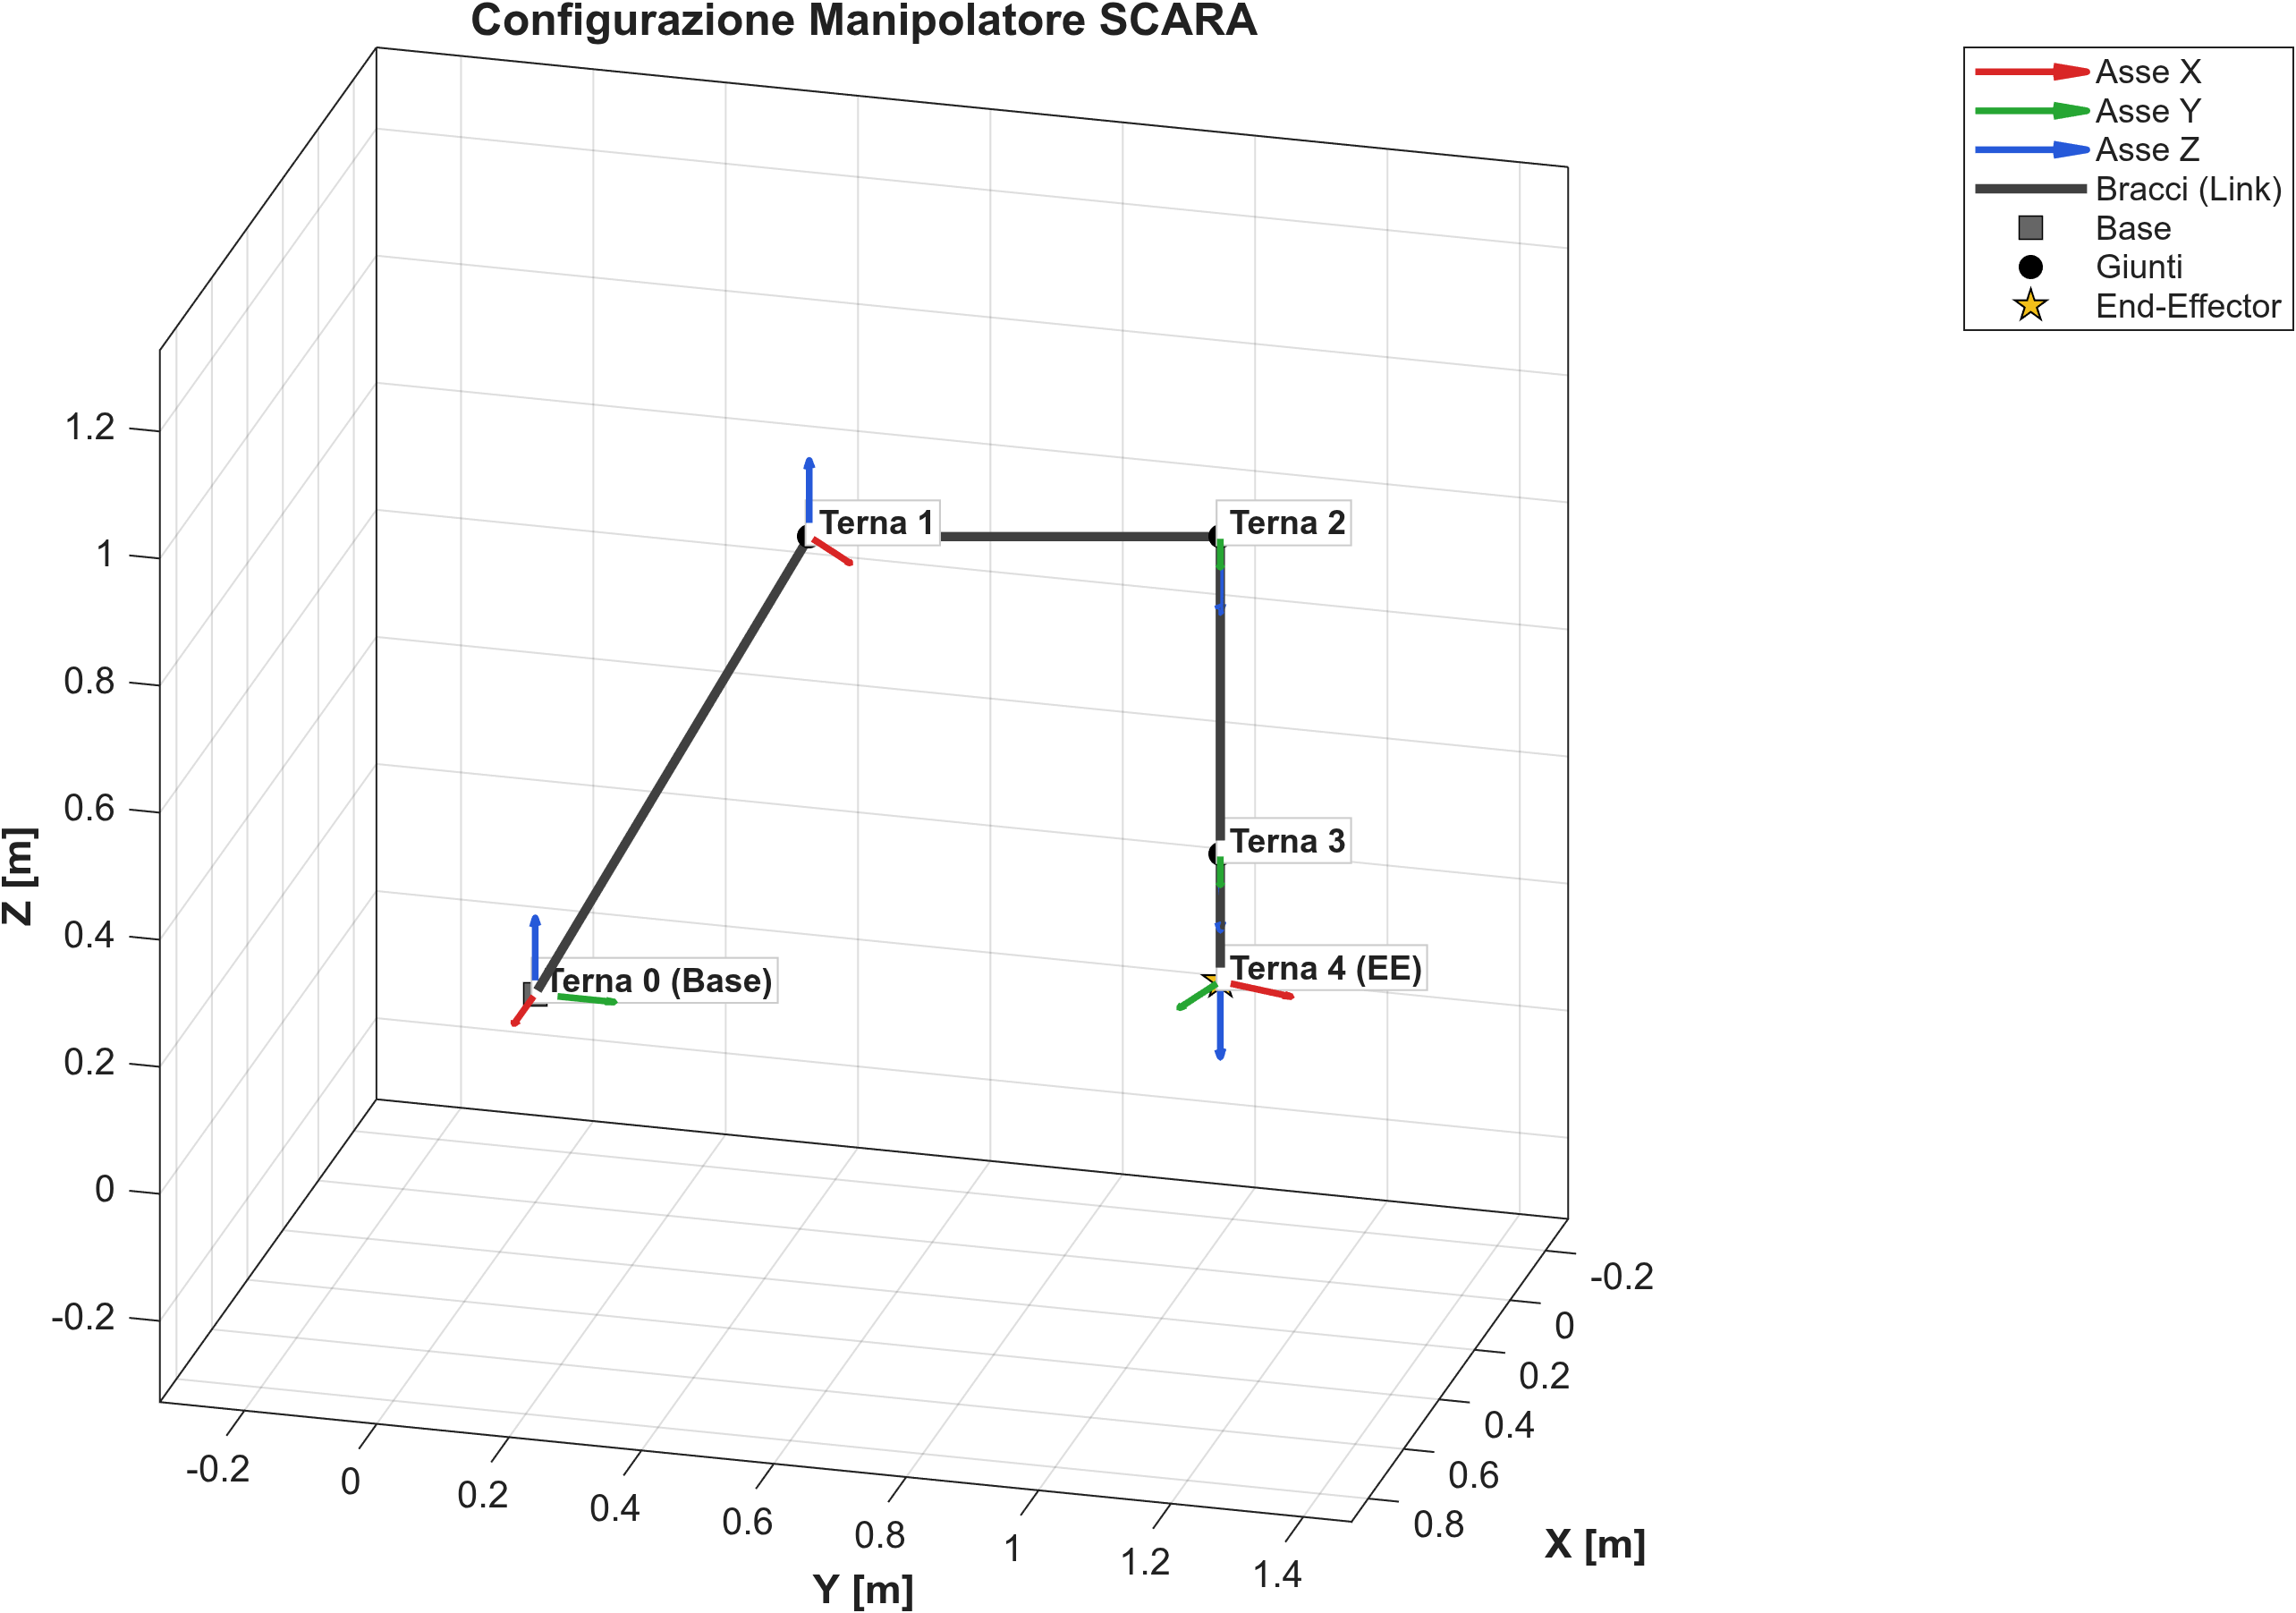
\includegraphics[width=1\linewidth]{E4_2_CinematicaDirettaManipolatoreSCARA.png}
\end{center}

\end{document}
